\documentclass[main]{subfiles}

\begin{document}

\tableofcontents
\newpage

\section{Manifold}

\begin{definition}
A \textit{submanifold}\index{Submanifold} $N$ is a inclusion and an immersion $i:N\hookrightarrow M$
\end{definition}

\begin{definition}
The kernel of $C^\infty_p(M)\to\mathbb R, f\mapsto f(p)$ is a maximal ideal $m_p$, define the \textit{cotangent space}\index{Cotangent space} $T^*_pM:=\dfrac{m_p}{m_p^2}$, for $f\in C^\infty(M)$, define $(df)_p=f-f(p)\mod m_p$, $(dx_1)_p,\cdots,(dx_n)_p$ form a basis of $T^*_pM$ locally, $(df)_p=\dfrac{\partial f}{\partial x_1}(p)(dx_1)_p+\cdots+\dfrac{\partial f}{\partial x_n}(p)(dx_n)_p$
\end{definition}

\begin{definition}
The \textit{tangent space}\index{Tangent space} $T_pM$ at $p$ are the derivations $Der(C^\infty_p(M))$ \par
$\left(\dfrac{\partial}{\partial x_1}\right)_p,\cdots,\left(\dfrac{\partial}{\partial x_n}\right)_p$ form a basis of $T_pM$ locally
\end{definition}

\begin{definition}
The \textit{pushforward(differential)}\index{Pushforward(differential)} of smooth map $\phi:M\to N$ is $\phi_p:T_pM\to T_pN$, $\phi_p(X_p)(f)=X_p(f\circ\phi)$
\end{definition}

\begin{definition}
The \textit{pullback}\index{Pullback} of smooth map $\phi:M\to N$ is $\phi^*:C^\infty(N)\to C^\infty(N)$, $\phi^*(f)=f\circ\phi$
\end{definition}

\begin{definition}
$\left(\varphi^*\alpha\right)_x(X)=\alpha_{\varphi(x)}(d\varphi_x(X))=\alpha_{\varphi(x)}((\varphi_*)_x(X))$, or in short $\varphi^*\alpha(X)=\alpha(\varphi_*X)$, similarly, for $k$ forms, $\varphi^*\alpha(X_1,\cdots, X_k)=\alpha(\varphi_*X_1,\cdots,\varphi_*X_k)$ \par
In particular, $\varphi^*(dx)=d(x\circ\varphi)$, pullback is compatible with wedge product, $\varphi^*(\alpha\wedge\beta)=\varphi^*\alpha\wedge\varphi^*\beta$, and pullback is compatible with exterior derivative, $\varphi^*(d\alpha)=d(\varphi^*\alpha)$
The exterior multiplication by $\alpha$ is $\beta\mapsto\alpha\wedge\beta$
The interior multiplication by $v\in TM$ is $v\mathrel{\lrcorner}:\omega(-)\mapsto\omega(v,-)$
\end{definition}

\begin{definition}
$\pi:T^*M\to M$ is the cotangent bundle, the \textit{tautological one form} or \textit{canonical one form}\index{Tautological one form} is $\pi^*\omega$
\end{definition}

\begin{definition}
Let $M$ be a smooth manifold, $X,Y\in C^\infty(M,TM)$ are vector fields, define Lie bracket\index{Lie bracket of vector fields} $[X,Y]\in C^\infty(M,TM)$, $[X,Y](f):=(XY-YX)(f)=X(Y(f))-Y(X(f))$
\end{definition}

\begin{remark}
Check from local coordinates, $X(Y(f))$ is not well defined
\end{remark}

\begin{definition}
Let $M,N$ be smooth manifolds, $f:M\to N$ is a smooth map, it is called an immersion if $df$ is injective at any point, it is called submersion if $df$ is surjective at any point
\end{definition}

\begin{theorem}\label{Constant rank mapping theorem}
Suppose $M,N$ are smooth manifolds with dimension $m,n$, $f:M\to N$ is a smooth map with constant rank $r$, then for any $p\in M$, denote $f(p)=q$, there are local charts $(p,U)$, $(q,V)$ such that $\chi_V\circ f\circ\chi_U(x_1,\cdots,x_m)=(x_1,\cdots,x_r,0,\cdots,0)$. Moreover, suppose $M$ is second countable, if $f$ is injective, then $f$ is a immersion, if $f$ is surjective, then $f$ is a submersion, if $f$ is bijective, then $f$ is a diffeomorphism
\end{theorem}

\begin{proof}
If $f$ is surjective but not a submersion, then $r<n$, but then by Theorem \ref{Baire category theorem}, $f$ can't be surjective which is a contradiction
\end{proof}

\begin{theorem}\label{Constant rank level set theorem}
Suppose $M,N$ are smooth manifolds with dimension $m,n$, $f:M\to N$ is a smooth map with constant rank $r$, then a level set $S=f^{-1}(c)$ is an embedded submanifold in $M$ of codimension $r$ with $f|_S$ being a proper map
\end{theorem}

\begin{proposition}
Let $G$ be a Lie group, $M,N$ be smooth manifolds with a $G$ action, and $G$ acts transitively on $M$, for any equivariant map $f:M\to N$, $f$ has constant rank
\end{proposition}

\begin{proof}
For any $x\in M$, denote $y=f(x)$, it suffices to show $\mathrm{rank}(df)_x=\mathrm{rank}(df)_{gx}$ since $G$ acts transitively on $M$, note that $f(gx)=gf(x)$, thus $fL_g=L_{g}f$, $(df)_{gx}(dL_g)_x=d(L_g)_y(df)_x$, and group actions are isomorphisms, we have $\mathrm{rank}(df)_x=\mathrm{rank}(df)_{gx}$
\end{proof}

\begin{theorem}[Stokes' theorem]\label{Stokes' theorem}
$\langle\partial\Omega,\omega\rangle=\langle\Omega,d\omega\rangle$, here $\langle\Omega,\omega\rangle=\displaystyle\int_\Omega\omega$
\end{theorem}

\begin{theorem}[de Rham's theorem]
$M$ is a smooth manifold. $H_{\mathrm{dR}}^p(X;\mathbb R)\xrightarrow{\cong} H^p(X;\mathbb R)$ is an isomorphism
\end{theorem}

\begin{proof}
Since $\mathbb R$ is a divisible abelian group, thus an injective $\mathbb Z$ module, hence $\Ext^1_{\mathbb Z}(A,\mathbb R)$, thus universal coefficient theorem gives exact sequence
\[0=\Ext^1_{\mathbb Z}(H_{p-1}(X;\mathbb Z),\mathbb R)\to H^p(M;\mathbb R)\to \Hom(H_p(X;\mathbb Z),\mathbb R)\to0\]
The isomorphism is given by $H_{\mathrm{dR}}^p(X;\mathbb R)\to \Hom(H_p(X),\mathbb R)$, $\omega\mapsto\displaystyle\int_{-}\omega$
\end{proof}

\begin{definition}
$E\to X$ is a vector bundle, a connection on $E$ is an $\mathbb R$ linear map
\[\nabla:\Gamma(E)\to\Gamma(T^*X\otimes E)\]
satisfying Leibniz rule $\nabla(f\sigma)=f\otimes\nabla\sigma+df\otimes\sigma$
\end{definition}

\begin{lemma}
$\nabla_X(\sigma)=(\nabla\sigma)(X)$ defines a covariant derivative, conversely, every covariant derivative is defined this way
\end{lemma}



\section{Differential geometry of surfaces}

\begin{definition}
A \textbf{differentiable surface} is an embedding $S\hookrightarrow\mathbb R^3$
\end{definition}

\begin{lemma}
$\gamma(t)$ is a geodesic iff $\ddot\gamma$ is parallel to the normal $\vec n$, meaning no acceleration in $S$ \par
A geodesic $\gamma$ on $S$ has constant speed \par
The geodesic curvature of a curve $\gamma$ is the curvature of the projection onto tangent plane, $\gamma$ is a geodesic iff the geodesic curvature of $\gamma$ is zero
\end{lemma}

\begin{proof}
$\dfrac{d}{dt}|\dot\gamma|^2=2\ddot\gamma\cdot\dot\gamma=0$
\end{proof}



\section{Connection and curvature}

\begin{definition}
The \textit{volume form}\index{Volume form} is $\sqrt{|\det g|}dx_i\wedge dx_j$, which happen to be $\star1$
\end{definition}

\begin{definition}
\textit{Hodge star}\index{Hodge star} is defined to be $\eta\wedge\star\xi=\langle\eta,\xi\rangle\omega$, $\omega$ is the volume form. Consider $(\alpha,\beta)=\int_X\alpha\wedge\star\beta$, $d^*=(-1)^{kl+1}\star d\star$ is the \textit{codifferential}\index{Codifferential} that $(d\alpha,\beta)=(\alpha,d^*\beta)$, $\Delta=dd^*+d^*d$ is the Laplacian
\end{definition}

\begin{definition}
An \textbf{affine connection}\index{Affine connection} is
\begin{align*}
\nabla:\Gamma(TM)\otimes\Gamma(TM)&\to\Gamma(TM) \\
(X,Y)&\mapsto\nabla_XY
\end{align*}satisfying
\begin{itemize}
\item $\nabla_{fX}Y=f\nabla_XY$, i.e. $\nabla$ is $C^\infty(M,\mathbb R)$ linear in the first variable
\item $\nabla_X(fY)=XfY+f\nabla_XY$, i.e. $\nabla$ satisfies Leibniz rule in the second variable
\end{itemize}
From this we can define covariant derivative $\nabla$, $\nabla_Xf=X_f$, $(\nabla_X\alpha)(Y)=\nabla_X(\alpha(Y))-\alpha(\nabla_XY)$, here $\alpha$ is a covector, similarly for any tensor, Write contraction $(\nabla T)(\alpha_1,\cdots,\alpha_m,X_1,\cdots,X_n,X)=(\nabla_XT)(\alpha_1,\cdots,\alpha_m,X_1,\cdots,X_n)$, $T$ is a tensor
\end{definition}

\begin{note}
$\nabla_X(\alpha(Y))=\nabla_X(\alpha)(Y)+\alpha(\nabla_XY)$
\end{note}

\begin{definition}
$\nabla$ is an affine connection, the \textbf{torsion tensor}\index{Torsion tensor} is
\[T(X,Y)=\nabla_XY-\nabla_YX-[X,Y]\]
\end{definition}

\begin{definition}
The Levi-Civita connection $\nabla$ is the one satisfying
\begin{itemize}
\item $\nabla_Zg(X,Y)=g(\nabla_ZX,Y)+g(X,\nabla_ZY)$, i.e. $\nabla g=0$
\item $\nabla_XY-\nabla_YX=[X,Y]$, i.e. $\nabla$ is torsion free
\end{itemize}
\end{definition}

\begin{definition}
$\nabla$ is the Levi-Civita connection, the Riemannian curvature tensor is $R_{XY}=[\nabla_X,\nabla_Y]-\nabla_{[X,Y]}$
\end{definition}

\begin{remark}
$X,Y$ are commuting vector fields around $x_0$, then $\dfrac{d}{ds}\dfrac{d}{dt}\tau_{sX}^{-1}\tau_{tY}^{-1}\tau_{sX}\tau_{tY}Z=R_{XY}Z$, $\tau$ is the parallel transport
\begin{figure}[h!]
\centering
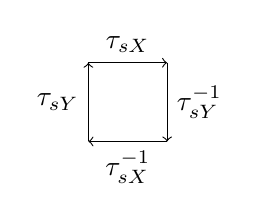
\begin{tikzpicture}
\draw[->](0,0)--(0,1);
\draw[->](0,1)--(1,1);
\draw[->](1,1)--(1,0);
\draw[->](1,0)--(0,0);
\node at (0.5,1)[above] {$\tau_{sX}$};
\node at (0,0.5)[left] {$\tau_{sY}$};
\node at (0.5,0)[below] {$\tau_{sX}^{-1}$};
\node at (1,0.5)[right] {$\tau_{sY}^{-1}$};
\end{tikzpicture}
\end{figure}
\end{remark}

\begin{definition}
$\nabla$ is a affine connection, denote $\partial_i=\frac{\partial}{\partial x_i}$, $g_{ij}=\langle\partial_i,\partial_j\rangle$, $\nabla_i=\nabla_{\partial_i}$. The \textit{Christoffel symbols}\index{Christoffel symbol} $\Gamma^k_{ij}$ is defined such that $\nabla_i\partial_j=\sum_{k}\Gamma^k_{ij}\partial_k$, then $\nabla_i\partial_j-\nabla_j\partial_i=\sum_k(\Gamma^k_{ij}-\Gamma^k_{ji})\partial_k$, if $\nabla$ is torsion free, then $\nabla_i\partial_j-\nabla_j\partial_i=[\partial_i,\partial_j]=0\Rightarrow\Gamma^k_{ij}=\Gamma^k_{ji}$. Since
\[\frac{\partial g_{ij}}{\partial x_k}=\nabla_kg_{ij}=\sum_{l}\Gamma^l_{ki}g_{jl}+\sum_{l}\Gamma^l_{kj}g_{il}\]
Switch $j,k$, we have
\[\frac{\partial g_{ik}}{\partial x_j}=\sum_{l}\Gamma^l_{ji}g_{kl}+\sum_{l}\Gamma^l_{kj}g_{il}\]
Then switch $i,j$, we have
\[\frac{\partial g_{jk}}{\partial x_i}=\sum_{l}\Gamma^l_{ij}g_{kl}+\sum_{l}\Gamma^l_{ki}g_{jl}\]
Thus
\[\frac{\partial g_{jk}}{\partial x_i}+\frac{\partial g_{ik}}{\partial x_j}-\frac{\partial g_{ij}}{\partial x_k}=2\sum_l\Gamma^l_{ij}g_{kl}\]
Therefore
\[\Gamma^k_{ij}=\frac{1}{2}\sum_lg^{kl}\left(\frac{\partial g_{jk}}{\partial x_i}+\frac{\partial g_{ik}}{\partial x_j}-\frac{\partial g_{ij}}{\partial x_k}\right)\]
\end{definition}

\begin{proposition} \hfill
\begin{enumerate}[leftmargin=*,label=\textbf{\arabic*.}]
\item $R_{YX}=-R_{XY}$
\item $(R_{XY}Z,W)=-(R_{XY}W,Z)$
\item $R_{XY}Z+R_{YZ}X+R_{ZX}Y=0$
\item 
\end{enumerate}
The \textbf{second Bianchi identity}\index{Second Bianchi identity} follows
\[\nabla_XR_{YZ}+\nabla_YR_{ZX}+\nabla_ZR_{XY}=0\]
\end{proposition}

\begin{remark}
If write $(R_{XY}Z,W)=R(X,Y,Z,W)$, then $R$ is antisymmetric about the first two variables and the last two variables, $R$ satisfies Jacobi identity, the first two and the last two variables can switch place
\end{remark}

\begin{proof}
\begin{enumerate}[leftmargin=*,label=\textbf{\arabic*.}]
\item 
\item 
\item 
\item Follow from above
\end{enumerate}
\end{proof}

\begin{definition}
There is a unique way to define the connection on all $(r,s)$ tensors that are compatible with tensor products(Leibniz rule) and tensor contraction. In particular we would have
\[\nabla_X(\omega(Y))=(\nabla_X\omega)(Y)+\omega(\nabla_XY)\]
Hence we have
\[\nabla dx_i=-\sum_{j,k}\Gamma_{kj}^idx_k\otimes dx_j\]
\end{definition}

\begin{definition}
$\{e_i\}$ is an orthonomal basis, the \textbf{Ricci curvature}\index{Ricci curvature} is $\Ric(X)=\sum R_{X,e_i}e_i$. The \textbf{scalar curvature}\index{Scalar curvature} is $S=\Tr\Ric=\sum(\Ric(e_j),e_j)=\sum(R_{e_j,e_i}e_i,e_j)$. The \textbf{Einstein curvature}\index{Einstein curvature} is $G=R-\frac{1}{2}gS$
\end{definition}

\begin{definition}
The gradient $\grad f$ of a function $f$ is defined so that $g(\grad f, X)=Xf$. Assume $\grad f=Y$, $\sum_ig_{ik}Y_i=\frac{\partial f}{\partial x_k}$, suppose $(g^{ij})$ is the inverse of $(g_{ij})$, then $Y_j=\sum_i\frac{\partial f}{\partial x_i}g^{ij}$, $\grad f=\sum_j\left(\sum_i\frac{\partial f}{\partial x_i}g^{ij}\right)\frac{\partial}{\partial x_j}$
\end{definition}

\begin{definition}
The Hessian $\Hess f$ of a function $f$ is $\nabla^2 f$, or defined through $\Hess f(X,Y)=g(\nabla_X\grad f,Y)$. In local coordinates, we have
\begin{align*}
\nabla^2 f&=\nabla(df)=\sum_i\nabla\left(\frac{\partial f}{\partial x_i}dx_i\right)\\
&=\sum_i\nabla\left(\frac{\partial f}{\partial x_i}\right)\otimes dx_i+\sum_i\frac{\partial f}{\partial x_i}\nabla dx_i\\
&=\sum_{i,j}\frac{\partial^2f}{\partial x_i\partial x_j}dx_j\otimes dx_i-\sum_{i,j,k}\frac{\partial f}{\partial x_i}\Gamma_{kj}^idx_k\otimes dx_j\\
&=\sum_{i,j}\frac{\partial^2f}{\partial x_i\partial x_j}dx_i\otimes dx_j-\sum_{i,j,k}\frac{\partial f}{\partial x_k}\Gamma_{ij}^kdx_i\otimes dx_j\\
&=\sum_{i,j}\left(\frac{\partial^2f}{\partial x_i\partial x_j}-\sum_{k}\frac{\partial f}{\partial x_k}\Gamma_{ij}^k\right)dx_i\otimes dx_j
\end{align*}
In other words, $\Hess f(X,Y)=X(Yf)-(\nabla_XY)f$
\end{definition}

\begin{definition}[Musical isomorphisms]
$\sharp:T^*M\to TM, \flat:TM\to T^*M$. $(\omega^\sharp,X)=\omega(Y)$, $(X^\flat,\alpha)=\alpha(X)$. For example, $dx_i^\sharp=\sum_kg^{ik}\frac{\partial}{\partial x_k}$
\end{definition}

Riemann metric induces an inner product on $T^*M$ through musical isomorphisms. For example, $(dx_i,dx_j)=(dx_i^\sharp,dx_j^\sharp)=\sum_{kl}g^ikg^{jl}\left(\frac{\partial}{\partial x_k},\frac{\partial}{\partial x_l}\right)=\sum_{kl}g^{ik}g^{lj}g^{kl}=g^{ij}$. This also gives an inner product on $T^k_M$

\begin{definition}
The Laplacian $\Delta f=\tr\Hess f$ is the trace of the Hessian. Here the trace is the trace contraction taken with respect to the metric. In local coordinates
\[\Delta f=\sum_{i,j}g^{ij}\left(\frac{\partial^2f}{\partial x_i\partial x_j}-\sum_{k}\frac{\partial f}{\partial x_k}\Gamma_{ij}^k\right)\]
\end{definition}



\section{Hyperbolic geometry}

\begin{definition}
$\mathbb R^{n+1}$ with metric $ds^2=dx_1^2+\cdots+dx_n^2-dx_0^2$ is the \textit{Minkowski space}\index{Minkowski space} \par
The \textbf{hyperboloid model}\index{Hyperboloid model} is $\mathbb H=\{x_1^2+\cdots+x_n^2-x_0^2=-1,x_0>0\}$. The Riemannian metric is the pullback metric $ds^2=dx_1^2+\cdots+dx_n^2-dx_0^2$ \par
The geodesics are intersections of $\mathbb H$ and two dimensional subspaces of $\mathbb R^{n+1}$
$(d\sinh s)^2+(d\cosh s)^2=\cosh^2sds^2-\sinh^2sds^2=ds^2$, thus $\mathbb H^1$ is isomorphic to $\mathbb E^1$
\begin{center}
\begin{tikzpicture}[scale=2]
% \draw[dashed] (-2,2)--(0,0)--(2,2);
\draw[ultra thick,blue,smooth,samples=100,domain=-1.5:1.5] plot({sinh((\x))},{cosh((\x))});
\node[blue] at (2,2) [right]{Hyperboloid model};
\begin{scope}
\clip(-1,0) rectangle (1,1);
\draw[ultra thick, red] (0,0)circle(1);
\end{scope}
\node[red] at (-1,0.5) [left]{Hemisphere model};
\draw[thin,->](-2,0)--(2,0) node[below] {$x'$};
\draw[thin,->](0,-1.5)--(0,2.5) node[right] {$x_0$};
\draw[ultra thick, yellow] (-1,1)--(1,1);
\node[yellow] at (-1,1) [left]{Klein disc model};
\draw[ultra thick, green] (-1,0)--(1,0);
\node[green] at (-1,-0.2) {Poincar\'e disc model};
\draw[ultra thick, brown] (1,-1.5)--(1,2.5);
\node[brown] at (1,0.5) [right]{Halfspace model};
\coordinate (A) at (1.1500299029183623,1.5239976304464578) ;
\coordinate (B) at (0.754613970483313,0.6561689992306932);
\coordinate (C) at (0.4556382656805185,0);
\coordinate (D) at (0.754613970483313,1);
\coordinate (E) at (1,0.7479354550561907);
\coordinate (F) at (0.754613970483313,0);
\filldraw (A) circle (0.02) node[below right] {$A$};
\filldraw (B) circle (0.02) node[below left] {$B$};
\filldraw (C) circle (0.02) node[below right] {$C$};
\filldraw  (D) circle (0.02) node[above] {$D$};
\filldraw  (E) circle (0.02) node[right] {$E$};
\draw[dashed] (A)--(0,0);
\draw[dashed] (A)--(0,-1);
\draw[dashed] (E)--(-1,0);
\draw[dashed] (D)--(F);
\draw[thin] ($(F)+(0,0.05)$)--($(F)+(0.05,0.05)$)--($(F)+(0.05,0)$);
\end{tikzpicture}
\end{center}
$(x',x_n)\mapsto\left(\dfrac{2x'}{1+x_n},1\right)$, $x'=(x_0,\cdots,x_{n-1})$ is the isometry from the hemisphere to the halfspace \par
$(x',1)\mapsto\left(\dfrac{4x'}{4+|x'|^2},\dfrac{4-|x'|^2}{4+|x'|^2}\right)$, $x'=(x_0,\cdots,x_{n-1})$ is the isometry from the halfspace to the hemisphere \par
$x\mapsto\left(\dfrac{x'}{1+x_0}\right)$, $x'=(x_1,\cdots,x_n)$ is the isometry from the hemisphere to Poincar\'e disc \par
$x\mapsto\left(\dfrac{2x}{1-|x|^2},\dfrac{1+|x|^2}{1-|x|^2}\right)$ is the isometry from Poincar\'e disc to the hyperboloid \par
$x\mapsto\left(1,x'\right)$, $x'=(x_1,\cdots,x_n)$ is the isometry from the hemisphere to Klein disc \par
$x\mapsto\left(\dfrac{x'}{x_0},\dfrac{1}{x_0}\right)$, $x'=(x_1,\cdots,x_n)$ is the isometry from the hyperboloid to the hemisphere \par
$x\mapsto\left(\dfrac{x'}{x_0},\dfrac{1}{x_0}\right)$, $x'=(x_1,\cdots,x_n)$ is the isometry from the hemisphere to the hyperboloid \\
$(x_0,x')\mapsto\left(1,\dfrac{x'}{x_0}\right)$ is the isometry from the hyperboloid to the Klein model \\
$(x,1)\mapsto\left(\dfrac{1}{\sqrt{1-|x|^2}},\dfrac{x}{\sqrt{1-|x|^2}}\right)$ is the isometry from the Klein model to the hyperboloid \\


The \textbf{hemisphere model}\index{Hemisphere model} is $\mathbb H=\{x_0>0\}\cap S^{n}$. The Riemannian metric is pullback metric
\begin{align*}
\sum_{i=0}^{n-1}\left[d\left(\frac{x_i}{x_n}\right)\right]^2-\left[d\left(\frac{1}{x_n}\right)\right]^2
&=\sum_{i=0}^{n-1}\left(\frac{x_0dx_i-x_idx_0}{x_0^2}\right)^2-\left(-\frac{dx_0}{x_0^2}\right)^2 \\
&=\sum_{i=0}^{n-1}\frac{x_0^2dx_i^2-2x_ix_0dx_idx_0+x_i^2dx_0^2}{x_0^4}-\frac{dx_0^2}{x_0^4} \\
&=\frac{dx'^2}{x_0^2}-\frac{d(|x'|^2)d(x_0^2)}{2x_0^4}+\frac{|x'|^2dx_0^2-dx_0^2}{x_0^4} \\
&=\frac{dx'^2}{x_0^2}-\frac{d(1-x_0^2)d(x_0^2)}{2x_0^4}-\frac{dx_0^2}{x_0^2} \\
&=\frac{dx'^2}{x_0^2}+\frac{2dx_0^2}{x_0^2}-\frac{dx_0^2}{x_0^2} \\
&=\frac{dx'^2+dx_0^2}{x_0^2}
\end{align*}
The \textbf{half space model}\index{Half space model} is $\mathbb H=\{x_0>0\}\cap\{x_n=1\}$. The Riemannian metric is pullback metric
\begin{align*}
\frac{\displaystyle\sum_{i=0}^{n-1}d\left(\dfrac{4x_i}{4+|x'|^2}\right)^2+d\left(\dfrac{4-|x'|^2}{4+|x'|^2}\right)^2}{\left(\dfrac{4x_0}{4+|x'|^2}\right)^2}
&\xequal{X=4+|x'|^2}
\frac{\displaystyle\sum_{i=0}^{n-1}d\left(\dfrac{4x_i}{X}\right)^2+d\left(\dfrac{8}{X}-1\right)^2}{\left(\dfrac{4x_0}{X}\right)^2} \\
&=\frac{X^2}{x_0^2}\left(\displaystyle\sum_{i=0}^{n-1}d\left(\dfrac{x_i}{X}\right)^2+4d\left(\dfrac{1}{X}\right)^2\right) \\
&=\frac{X^2}{x_0^2}\left(\displaystyle\sum_{i=0}^{n-1}\left(\dfrac{Xdx_i-x_idX}{X^2}\right)^2+4\dfrac{dX^2}{X^4}\right) \\
&=\frac{1}{x_0^2}\left(\displaystyle\sum_{i=0}^{n-1}\dfrac{X^2dx_i^2+x_i^2dX^2-2Xx_idXdx_i}{X^2}+4\dfrac{dX^2}{X^2}\right) \\
&=\frac{1}{x_0^2}\left(dx'^2+\dfrac{|x'|^2dX^2}{X^2}+\dfrac{4dX^2}{X^2}-\dfrac{dXd(|x'|^2)}{X}\right) \\
&=\frac{1}{x_0^2}\left(dx'^2+\dfrac{XdX^2}{X^2}-\dfrac{dXd(X-4)}{X}\right) \\
&=\frac{dx'^2}{x_0^2} \\
\end{align*}
The \textbf{Poincar\'e disc model}\index{Poincar\'e disc model} is $\mathbb H=D^n$. The Riemannian metric is pullback metric
\begin{align*}
\sum_{i=1}^nd\left(\dfrac{2x_i}{1-|x|^2}\right)^2-d\left(\dfrac{1+|x|^2}{1-|x|^2}\right)^2
&\xequal{X=1-|x'|^2}
\sum_{i=1}^nd\left(\dfrac{2x_i}{X}\right)^2-d\left(\dfrac{2}{X}-1\right)^2 \\
&=4\sum_{i=1}^n\left(\dfrac{Xdx_i+x_idX}{X^2}\right)^2-4\left(-\dfrac{dX}{X^2}\right)^2 \\
&=4\sum_{i=1}^n\dfrac{X^2dx_i^2+x_i^2dX^2-Xx_idXdx_i}{X^4}-4\dfrac{dX^2}{X^4} \\
&=4\left(\dfrac{dx^2}{X^2}+\dfrac{|x|^2dX^2}{X^4}-\dfrac{dX^2}{X^4}-\dfrac{d(|x|^2)dX}{X^3}\right) \\
&=4\left(\dfrac{dx^2}{X^2}-\dfrac{XdX^2}{X^4}-\dfrac{d(1-X)dX}{X^3}\right) \\
&=\frac{4dx^2}{X^2}=\frac{4dx^2}{(1-|x|^2)^2}
\end{align*}

The \textbf{Klein disc model}\index{Klein disc model} is $\mathbb H=D^n$. The Riemannian metric is
\[\left|d\left(\frac{x}{\sqrt{1-|x|^2}}\right)\right|^2-d\left(\frac{1}{\sqrt{1-|x|^2}}\right)^2=\frac{|dx|^2}{1-|x|^2}+\frac{(x\cdot dx)^2}{(1-|x|^2)^2}=\sum\frac{(1-|x|^2+x_i^2)}{(1-|x|^2)^2}dx_i^2\]
The distance between $P,Q$ is $\dfrac{1}{2}\ln\left(\dfrac{|XQ||PY|}{|XY||PQ|}\right)=\dfrac{1}{2}\ln\left(X,P;Q,Y\right)$, $(X,P;Q,Y)$ is the cross ratio
\begin{center}
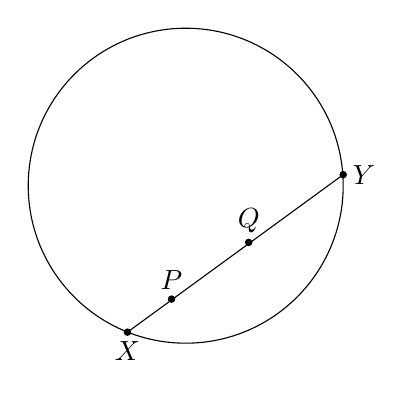
\begin{tikzpicture}[scale=2]
\draw (0,0) circle (1);
\coordinate (X) at (-0.37,-0.93);
\coordinate (P) at (-0.09,-0.72);
\coordinate (Q) at (0.4,-0.36);
\coordinate (Y) at (1,0.07);
\filldraw (X) circle (0.02) node[below] {$X$};
\filldraw (P) circle (0.02) node[above] {$P$};
\filldraw (Q) circle (0.02) node[above] {$Q$};
\filldraw (Y) circle (0.02) node[right] {$Y$};
\draw (X)--(Y);
\end{tikzpicture}
\end{center}
\end{definition}

\begin{theorem}
$\Isom(\mathbb H^2)=PSL(2,\mathbb R)$
\end{theorem}

\begin{proof}
An isometry sends half circles and orthogonal lines to half circles or orthogonal lines, by Schwarz reflection principle \ref{Schwarz reflection principle}, it is can be regard as an isometry on $\mathbb CP^1$ sending $\mathbb RP^1$ to $\mathbb RP^1$, then it necessarily has to be in $PSL(2,\mathbb R)$
\end{proof}

\begin{theorem}
$\Isom(\mathbb H^3)=PSL(2,\mathbb C)\ltimes\mathbb Z/2\mathbb Z\cong SL(2,\mathbb C)$
\end{theorem}

\begin{proof}
Since $\partial\mathbb H^3$ is the Riemann sphere, every isometry on $\mathbb H^3$ restricts to a conformal map on $\partial\mathbb H^3$ because it sends hemispheres and orthogonal planes to hemispheres or orthogonal planes, hence it is a M\"obius transformation. On the other hand, M\"obius transformations which can all be extended to an isometry on $\mathbb H^3$, translations $z\mapsto z+\lambda$ can be extended to $(z,x_3)\mapsto(z+\lambda,x_3)$, dilations $z\mapsto\lambda z$ can be extended to $(z,x_3)\mapsto (\lambda z,|\lambda|x_3)$, inversions $z\mapsto -\dfrac{1}{z}$ can be extended to $(z,x_3)\mapsto\left(\dfrac{-\bar z}{|z|^2+x_3^2},\dfrac{x_3}{|z|^2+x_3^2}\right)$. Therefore the isometry group for $\mathbb H^3$ is $PSL(2,\mathbb C)\ltimes\mathbb Z/2\mathbb Z\cong SL(2,\mathbb C)$
\end{proof}



\section{Complex manifold}

Suppose $\langle,\rangle$ is a Hermitian inner product on $\mathbb C^n$, then $\operatorname{Re}\langle,\rangle$ is a real inner product on $\mathbb R^{2n}$, i.e. $\operatorname{Re}\langle X_1+iX_2,Y_1+iY_2\rangle=\operatorname{Re}\langle X_1,Y_1\rangle+\operatorname{Re}\langle X_2,Y_2\rangle$. On the other hand, a inner product on $\mathbb R^n$ can be extended to a Hermitian inner product on the complexification $\mathbb C^n$ by complex linearality

\begin{definition}
$M$ is an even dimensional real manifold, an \textit{almost complex structure}\index{Almost complex structure} is $J:T_{\mathbb R}M\to T_{\mathbb R}M$ such that $J^2=-1_{T_{\mathbb R}M}$. A complex manifold has an almost complex structure
\[J\dfrac{\partial}{\partial x_i}=\dfrac{\partial}{\partial y_i}, J\dfrac{\partial}{\partial y_i}=-\dfrac{\partial}{\partial x_i}\]
\end{definition}

\begin{example}
$S^4$ cannot be given an almost complex structure. $S^6$ can be given an almost complex structure but not a complex structure
\end{example}

\begin{definition}
$A$ is a $(1,1)$ form, the Nijenhuis tensor is
\[N_A(X,Y)=-A^2[X,Y]+A([AX,Y]+[X,AY])-[AX,AY]\]
\end{definition}

\begin{theorem}[Newslander-Nirenberg theorem]
$J$ is \textit{integrable} iff $N_J=0$. Meaning there is a unique complex structure which will give $J$
\end{theorem}

\begin{proposition}
Given an almost complex structure, we can find coordinate charts $(z_1,\cdots,z_n,\bar z_1,\cdots,\bar z_n)$ such that $\Span\left\{\dfrac{\partial}{\partial z_i}\right\}$, $\Span\left\{\dfrac{\partial}{\partial \bar z_i}\right\}$ to be the $i$ and $-i$ eigenspaces of $J$
\end{proposition}

\begin{definition}
A \textit{Hermitian manifold}\index{Hermitian manifold} $M$ is a complex manifold with a \textit{Hermitian metric}\index{Hermitian metric} $h=\sum h_{\alpha\bar\beta}dz_\alpha \otimes d\bar z_\beta$ on $TM\otimes\mathbb C$, where $h_{\alpha\bar\beta}$ is a positive definite Hermitian matrix. The real part gives a Riemannian metric
\begin{align*}
g&=\dfrac{1}{2}(h+\bar h) \\
&=\dfrac{1}{2}\left(\sum h_{\alpha\bar\beta}dz_\alpha \otimes d\bar z_\beta+\sum h_{\beta\bar\alpha}d\bar z_\alpha \otimes dz_\beta\right) \\
&=\frac{1}{2}\sum h_{\alpha\bar\beta}(dz_\alpha \otimes d\bar z_\beta+d\bar z_\beta \otimes dz_\alpha) \\
&=\sum h_{\alpha\bar\beta}dz_\alpha d\bar z_\beta
\end{align*}
Also gives \textit{associate} $(1,1)$ \textit{form}\index{Associate $(1,1)$ form}
\[\omega=-\dfrac{h-\bar h}{2i}=\dfrac{i}{2}(h-\bar h)=\dfrac{i}{2}\sum h_{\alpha\bar\beta}(dz_\alpha\otimes d\bar z_\beta-d \bar z_\beta\otimes dz_\alpha)=\frac{i}{2}\sum h_{\alpha\bar\beta}dz_\alpha\wedge d\bar z_\beta\]
Note that the volume form is $\vol_M=\dfrac{\omega^{\wedge n}}{n!}$
\end{definition}

\begin{remark}
$\omega(u,v)=g(Ju,v)$, $h=g-i\omega$, $g(u,v)=\omega(u,Jv)$. Any one determines the other two. $\omega$ corresponds to \textit{K\"ahler class}\index{K\"ahler class} in $H^2(M,\mathbb R)$
\end{remark}

\begin{definition}
A Hermitian manifold $M$ is a \textit{K\"ahler manifold}\index{K\"ahler manifold} if $d\omega=0$, $\omega$ is called the \textit{K\"ahler form}\index{K\"ahler form}. A symplectic manifold $(M,\omega)$ with an almost complex structrue $J$ is a Kahler manifold if $\omega(Ju,Jv)=\omega(u,v)$ and $g(u,v)=\omega(u,Jv)$ is a Riemannian metric. An even dimensional Riemannian manifold $(M,g)$ with an almost complex structure $J$ is a Kahler manifold if $g(Ju,Jv)=g(u,v)$ and $J$ is preserved by parallel transport, i.e. $\nabla J=0$

Since $\omega$ is a real form, thus by Poincare's lemma, $\omega=d\alpha$ for some $\alpha=\beta+\bar\beta$, where $\beta$ is a $(1,0)$ form, then we have $\partial\beta=\bar\partial\bar\beta=0$, hence $\omega=\partial\bar\beta+\bar\partial\beta$, $\beta=\partial\phi$, $\omega=\partial\bar\partial(\bar\phi-\phi)$. We have $\partial_{\gamma}h_{\alpha\bar\beta}=\partial_{\alpha}h_{\gamma\bar\beta}$, $\partial_{\bar\gamma}h_{\alpha\bar\beta}=\partial_{\bar\beta}h_{\alpha\bar\gamma}$, this implies at least locally $h_{\alpha\bar\beta}=\partial_\alpha f_{\bar\beta}$, and then $\partial_\alpha\partial_{\bar\gamma}f_{\bar\beta}=\partial_{\bar\gamma}\partial_\alpha f_{\bar\beta}=\partial_{\bar\beta}\partial_\alpha f_{\bar\gamma}=\partial_\alpha\partial_{\bar\beta}f_{\bar\gamma}$, hence $h_{\alpha\bar\beta}=\partial_\alpha\partial_{\bar\beta}\rho$, $\rho$ is called the local \textit{K\"ahler potential}\index{K\"ahler potential}, $\rho$ is a K\"ahler potential if $\omega=\dfrac{i}{2}\partial\bar\partial\rho$
\end{definition}

\begin{definition}
Consider $L=\omega\wedge-:H^k(M)\to H^{k+2}(M)$, the \textit{primitive cohomology} is
\[P^{n-k}(M)=\ker\left(H^{n-k}(M)\xrightarrow{L^{k+1}}H^{n+k+2}(M)\right)\]
The \textit{hard Lefschetz theorem} says
\[H^n(M)=\bigoplus L^kP^{n-2k}(M)\]
\end{definition}

\begin{theorem}[Serre duality]\label{Serre duality}\index{Serre duality}
$X$ is complex manifold of complex dimension $n$, $E\to X$ is a holomorphic vector bundle, then we have
\[H^i(X,E)\cong H^{n-i}(X,K\otimes E^*)^*\]
Where $K:=\bigwedge^n T^*X$ is the canonical bundle \par
For example, if $X$ is a Riemann surface, $E=\mathcal{O}$, then $H^1(X,\mathcal{O})\cong H^0(X,K\otimes\mathcal{O})^*\cong H^0(X,\Omega)^*=\Omega(X)^*$
\end{theorem}



\section{Symplectic manifold}

\begin{definition}
$M$ is a smooth manifold, a \textit{symplectic structure}\index{Symplectic structure} on $M$ is a $2$ form $\omega$ that is nondegenerate and anti-symmetric on $T_pM$
\end{definition}

\end{document}